% Metódy inžinierskej práce

\documentclass[10pt,twoside,slovak,a4paper]{coursepaper}

\usepackage[slovak]{babel}
%\usepackage[T1]{fontenc}
\usepackage[IL2]{fontenc} % lepšia sadzba písmena Ľ než v T1
\usepackage[utf8]{inputenc}
\usepackage{graphicx}
\usepackage{url} % príkaz \url na formátovanie URL
\usepackage{hyperref} % odkazy v texte budú aktívne (pri niektorých triedach dokumentov spôsobuje posun textu)

\usepackage{cite}
%\usepackage{times}

\pagestyle{headings}

\title{Hry pre zdravie ako súčasť každodenného života\thanks{Semestrálny projekt v predmete Metódy inžinierskej práce, ak. rok 2022/23, vedenie: Ing.Igor Stupavský}} % meno a priezvisko vyučujúceho na cvičeniach

\author{Kristián Červenka\\[2pt]
	{\small Slovenská technická univerzita v Bratislave}\\
	{\small Fakulta informatiky a informačných technológií}\\
	{\small \texttt{xcervenkak@stuba.sk}}
	}

\date{\small 19. september 2022} % upravte



\begin{document}

\maketitle

\begin{abstract}
V tomto článku som sa preto rozhodol zamerať na vnášanie gamifikácie do oblasti zdravotníctva a využitie hier pre zdravie a ich vplyv v oblasti bežného života ľudí.
Objasním, čo sú to vlastne hry pre zdravie a ako vedia byť prospešné pre vývoj dieťaťa.
Ďalej by som sa chcel zamerať na zlepšenie životného štýlu používateľov hier pre to určených.Objasním hry pre zdravie na akom princípe fungujú a čo je zároveň ich cieľom.
Objasním princíp fungovania hier pre zdravie, ich cieľ a implementáciu v každodennom živote.
Spracujem tému ako sú hry jednou zo schopností ako prinútiť ľudí byť flexibilný , respektíve viacej sa hýbať v dnešnom technologickom svete a zároveň sa proaktívne vysporiadať s rýchlo meniacim svetom technológií. 
Hry sú jednou z možností ako zmeniť ľudské správanie na prijateľnejšie pre spoločnosť preto sa zameriam aj na hry pre psychické zdravie.
\end{abstract}



\section{Úvod}
Videohry ponúkajú inovatívne, vzrušujúce a vysoko efektívne metódy na zvyšovanie vedomostí a ovplyvňovanie zdravotných výsledkov. 
V 21.storočí rastie potreba chrániť zdravie ľudí prostredníctvom variácie dostupných zdrojov.
Jednou z možností ako zlepšiť zdravie ľudí pohybujúcich sa po tomto svete je zasadenie gamifikácie do prostredia zdravotníctva. 
Pre spracovanie témy som sa rozhodol z dôvodu nárastu dopytu hier hre zdravie.Videohry majú schopnosť zaujať používateľov inou cestou ako iné média.
V oblasti zdravotníctva sa videohry objavili v rôznych oblastiach. 
Za posledných dvadsať rokov sa používajú v odbornom výcviku, terapii, starostlivosti o seba, podpore zdravia i v komunikácii o zdraví.

~\ref{nejaka}.
Dôležité súvislosti sú uvedené v častiach~\ref{dolezita} a~\ref{dolezitejsia}.
Záverečné poznámky prináša časť~\ref{zaver}.



\section{Motivácia} 
\subsection{Hry pre zdravie}
Videohry vo všeobecnosti majú schopnosť zaujať hráčov ako iným spôsobom ako ponúkajú dnešné novodobé média.Hry sa stávajú zaujímavou oblasťou rôznych výskumov a pokusov predvádzaných vedcami. Zo štúdie asociovanej Entertainment Software Association \cite{PLP-Framework} vyplýva , že približne 29\% hráčov sú v rozmedzí 18 a menej rokov. 
V súčastnosti využívame sofistikované technológie na podporu zdravia spôsobom , ktorý bol nepredstaviteľný pre minulé generácie.Množstvo hier pre zdravie je postavených na platformách dávno známych hráčom , ako sú napríklad osobné počítače alebo webové stránky.Hry podnecujú ich používateľov k opakovanému hraniu a preukazujú postupné  pozitívne zmeny správania potrebné na dosiahnutie individuálnych zdravotných zmien.
\subsection{Moderné pokroky v oblasti hier pre zdravie}
Vývoj a testovanie prebieha v širokom spektre chorôb , na prevenciu a liečbu zdravotných problémov.Bolo vykonaných množstvo výskumov zameraných na zdravotný stav človeka, akými sú napríklad cystická fibróza,liečba bolesti , Parkinsonova choroba , obezita a rôzne variácie vírusových ochorení.Tento výskum zahŕňal mimo iných i psychické  choroby a rehabilitácie, akými sú napríklad depresia, posttraumatická stresová porucha , úzkosť , popáleniny , mŕtvica,traumatické poškodenia mozgu a mnohé iné.Príkladom sú sociálne problémy , s ktorými sa ľudstvo stretáva takmer každý deň, násilie , šikanovanie , rasové predsudky\cite{bworld}.







\label{nejaka}
\section{Modifikácie hier pre zdravie v oblastiach bežného života}

\subsection{Hry ako forma edukácie prospešná pre vývoj dieťaťa}
Hry sú formou rekreácie, ktorá sa vo všeobecnosti považuje za prospešnú pre rozvoj dieťaťa. Vo väčšine prípadov majú hry pravidlá , ciele, možnosti voľby, výzvy a body , ktoré od mala nabádajú dieťa ku základným pravidlám spoločnosti. Príkladom sú seriózne hry , ktoré sú navrhnuté tak , aby mimo zábavy vniesli do života i iný účel.Tím vedcov zaoberajúcimi sa hrami o zdraví kategorizoval tieto hry do najmänej piatich kategórií.
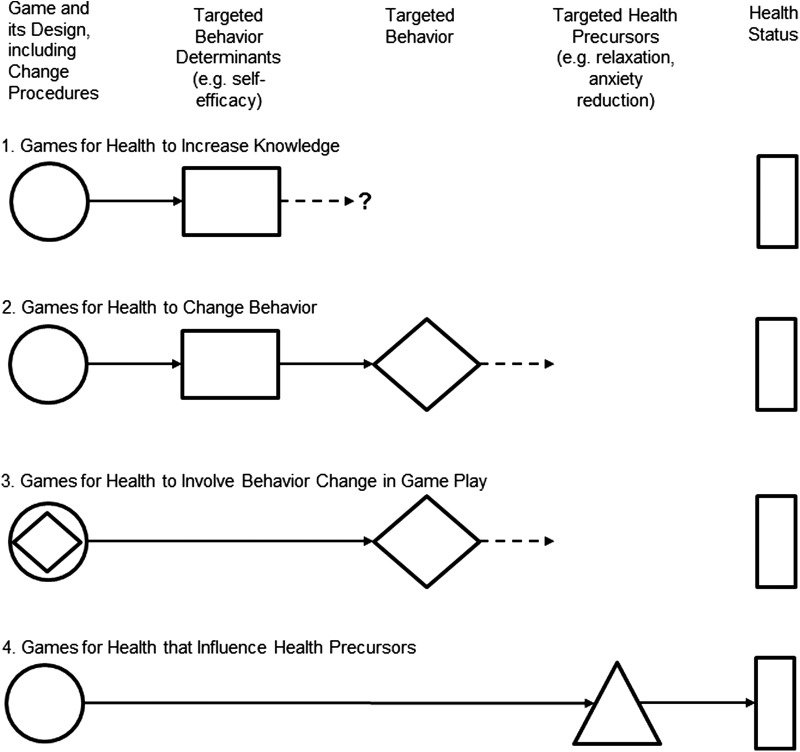
\includegraphics[scale=1.5]{tps_1.jpeg}
\subsubsection{Podsekcia podsekcie 1}

Z obr.~\ref{f:rozhod} je všetko jasné. 

\begin{figure*}[tbh]
\centering
%\includegraphics[scale=1.0]{diagram.pdf}
Aj text môže byť prezentovaný ako obrázok. Stane sa z neho označný plávajúci objekt. Po vytvorení diagramu zrušte znak \texttt{\%} pred príkazom \verb|\includegraphics| označte tento riadok ako komentár (tiež pomocou znaku \texttt{\%}).
\caption{Rozhodujúci argument.}
\label{f:rozhod}
\end{figure*}



\section{Iná časť} \label{ina}

Základným problémom je teda\ldots{} Najprv sa pozrieme na nejaké vysvetlenie (časť~\ref{ina:nejake}), a potom na ešte nejaké (časť~\ref{ina:nejake}).\footnote{Niekedy môžete potrebovať aj poznámku pod čiarou.}

Môže sa zdať, že problém vlastne nejestvuje\cite{Coplien:MPD}, ale bolo dokázané, že to tak nie je~\cite{Czarnecki:Staged, Czarnecki:Progress}. Napriek tomu, aj dnes na webe narazíme na všelijaké pochybné názory\cite{PLP-Framework}. Dôležité veci možno \emph{zdôrazniť kurzívou}.


\subsection{Nejaké vysvetlenie} \label{ina:nejake}

Niekedy treba uviesť zoznam:

\begin{itemize}
\item jedna vec
\item druhá vec
	\begin{itemize}
	\item x
	\item y
	\end{itemize}
\end{itemize}

Ten istý zoznam, len číslovaný:

\begin{enumerate}
\item jedna vec
\item druhá vec
	\begin{enumerate}
	\item x
	\item y
	\end{enumerate}
\end{enumerate}


\subsection{Ešte nejaké vysvetlenie} \label{ina:este}

\paragraph{Veľmi dôležitá poznámka.}
Niekedy je potrebné nadpisom označiť odsek. Text pokračuje hneď za nadpisom.



\section{Dôležitá časť} \label{dolezita}
\cite{Coplien:MPD}




\section{Ešte dôležitejšia časť} \label{dolezitejsia}




\section{Záver} \label{zaver} % prípadne iný variant názvu



%\acknowledgement{Ak niekomu chcete poďakovať\ldots}


% týmto sa generuje zoznam literatúry z obsahu súboru literatura.bib podľa toho, na čo sa v článku odkazujete
\bibliography{literatura.bib}
\bibliographystyle{abbrv} % prípadne alpha, abbrv alebo hociktorý iný
\end{document}
